\documentclass[twoside]{book}

% Packages required by doxygen
\usepackage{fixltx2e}
\usepackage{calc}
\usepackage{doxygen}
\usepackage[export]{adjustbox} % also loads graphicx
\usepackage{graphicx}
\usepackage[utf8]{inputenc}
\usepackage{makeidx}
\usepackage{multicol}
\usepackage{multirow}
\PassOptionsToPackage{warn}{textcomp}
\usepackage{textcomp}
\usepackage[nointegrals]{wasysym}
\usepackage[table]{xcolor}

% Font selection
\usepackage[T1]{fontenc}
\usepackage[scaled=.90]{helvet}
\usepackage{courier}
\usepackage{amssymb}
\usepackage{sectsty}
\renewcommand{\familydefault}{\sfdefault}
\allsectionsfont{%
  \fontseries{bc}\selectfont%
  \color{darkgray}%
}
\renewcommand{\DoxyLabelFont}{%
  \fontseries{bc}\selectfont%
  \color{darkgray}%
}
\newcommand{\+}{\discretionary{\mbox{\scriptsize$\hookleftarrow$}}{}{}}

% Page & text layout
\usepackage{geometry}
\geometry{%
  a4paper,%
  top=2.5cm,%
  bottom=2.5cm,%
  left=2.5cm,%
  right=2.5cm%
}
\tolerance=750
\hfuzz=15pt
\hbadness=750
\setlength{\emergencystretch}{15pt}
\setlength{\parindent}{0cm}
\setlength{\parskip}{3ex plus 2ex minus 2ex}
\makeatletter
\renewcommand{\paragraph}{%
  \@startsection{paragraph}{4}{0ex}{-1.0ex}{1.0ex}{%
    \normalfont\normalsize\bfseries\SS@parafont%
  }%
}
\renewcommand{\subparagraph}{%
  \@startsection{subparagraph}{5}{0ex}{-1.0ex}{1.0ex}{%
    \normalfont\normalsize\bfseries\SS@subparafont%
  }%
}
\makeatother

% Headers & footers
\usepackage{fancyhdr}
\pagestyle{fancyplain}
\fancyhead[LE]{\fancyplain{}{\bfseries\thepage}}
\fancyhead[CE]{\fancyplain{}{}}
\fancyhead[RE]{\fancyplain{}{\bfseries\leftmark}}
\fancyhead[LO]{\fancyplain{}{\bfseries\rightmark}}
\fancyhead[CO]{\fancyplain{}{}}
\fancyhead[RO]{\fancyplain{}{\bfseries\thepage}}
\fancyfoot[LE]{\fancyplain{}{}}
\fancyfoot[CE]{\fancyplain{}{}}
\fancyfoot[RE]{\fancyplain{}{\bfseries\scriptsize Generated by Doxygen }}
\fancyfoot[LO]{\fancyplain{}{\bfseries\scriptsize Generated by Doxygen }}
\fancyfoot[CO]{\fancyplain{}{}}
\fancyfoot[RO]{\fancyplain{}{}}
\renewcommand{\footrulewidth}{0.4pt}
\renewcommand{\chaptermark}[1]{%
  \markboth{#1}{}%
}
\renewcommand{\sectionmark}[1]{%
  \markright{\thesection\ #1}%
}

% Indices & bibliography
\usepackage{natbib}
\usepackage[titles]{tocloft}
\setcounter{tocdepth}{3}
\setcounter{secnumdepth}{5}
\makeindex

% Hyperlinks (required, but should be loaded last)
\usepackage{ifpdf}
\ifpdf
  \usepackage[pdftex,pagebackref=true]{hyperref}
\else
  \usepackage[ps2pdf,pagebackref=true]{hyperref}
\fi
\hypersetup{%
  colorlinks=true,%
  linkcolor=blue,%
  citecolor=blue,%
  unicode%
}

% Custom commands
\newcommand{\clearemptydoublepage}{%
  \newpage{\pagestyle{empty}\cleardoublepage}%
}

\usepackage{caption}
\captionsetup{labelsep=space,justification=centering,font={bf},singlelinecheck=off,skip=4pt,position=top}

%===== C O N T E N T S =====

\begin{document}

% Titlepage & ToC
\hypersetup{pageanchor=false,
             bookmarksnumbered=true,
             pdfencoding=unicode
            }
\pagenumbering{roman}
\begin{titlepage}
\vspace*{7cm}
\begin{center}%
{\Large Elgar Game Engine }\\
\vspace*{1cm}
{\large Generated by Doxygen 1.8.11}\\
\end{center}
\end{titlepage}
\clearemptydoublepage
\tableofcontents
\clearemptydoublepage
\pagenumbering{arabic}
\hypersetup{pageanchor=true}

%--- Begin generated contents ---
\chapter{Namespace Index}
\section{Namespace List}
Here is a list of all namespaces with brief descriptions\+:\begin{DoxyCompactList}
\item\contentsline{section}{\hyperlink{namespaceelgar}{elgar} }{\pageref{namespaceelgar}}{}
\end{DoxyCompactList}

\chapter{Class Index}
\section{Class List}
Here are the classes, structs, unions and interfaces with brief descriptions\+:\begin{DoxyCompactList}
\item\contentsline{section}{\hyperlink{classelgar_1_1Engine}{elgar\+::\+Engine} \\*Oversees all core functionalities of the Elgar pipeline. Every program using Elgar must utilize this class. (Note\+: Follows the singleton class design pattern) }{\pageref{classelgar_1_1Engine}}{}
\end{DoxyCompactList}

\chapter{File Index}
\section{File List}
Here is a list of all files with brief descriptions\+:\begin{DoxyCompactList}
\item\contentsline{section}{elgar/\hyperlink{Engine_8hpp}{Engine.\+hpp} }{\pageref{Engine_8hpp}}{}
\item\contentsline{section}{src/\hyperlink{Engine_8cpp}{Engine.\+cpp} }{\pageref{Engine_8cpp}}{}
\end{DoxyCompactList}

\chapter{Namespace Documentation}
\hypertarget{namespaceelgar}{}\section{elgar Namespace Reference}
\label{namespaceelgar}\index{elgar@{elgar}}
\subsection*{Classes}
\begin{DoxyCompactItemize}
\item 
class \hyperlink{classelgar_1_1Engine}{Engine}
\begin{DoxyCompactList}\small\item\em The \hyperlink{classelgar_1_1Engine}{Engine} class oversees all core functionalities of the Elgar pipeline. Every program using Elgar must utilize this class. (Note\+: Follows the singleton class design pattern) \end{DoxyCompactList}\end{DoxyCompactItemize}

\chapter{Class Documentation}
\hypertarget{classelgar_1_1Engine}{}\section{elgar\+:\+:Engine Class Reference}
\label{classelgar_1_1Engine}\index{elgar\+::\+Engine@{elgar\+::\+Engine}}


The \hyperlink{classelgar_1_1Engine}{Engine} class oversees all core functionalities of the Elgar pipeline. Every program using Elgar must utilize this class. (Note\+: Follows the singleton class design pattern)  




{\ttfamily \#include $<$Engine.\+hpp$>$}

\subsection*{Static Public Member Functions}
\begin{DoxyCompactItemize}
\item 
static void \hyperlink{classelgar_1_1Engine_ad7581c87901137b12fcbffe62ac711b1}{Init} ()
\begin{DoxyCompactList}\small\item\em Initializes Elgar and its subsystems and creates an instance of the engine. \end{DoxyCompactList}\item 
static void \hyperlink{classelgar_1_1Engine_a73d30730db3c8a9d132caa0c3cfe8e95}{Shutdown} ()
\begin{DoxyCompactList}\small\item\em Shuts down Elgar and its subsystems and destroys the engine instance. \end{DoxyCompactList}\item 
static \hyperlink{classelgar_1_1Engine}{Engine} $\ast$ \hyperlink{classelgar_1_1Engine_ac1cddebb329f111c5c084d7f0cb2f126}{Get\+Instance} ()
\begin{DoxyCompactList}\small\item\em Returns the Elgar \hyperlink{classelgar_1_1Engine}{Engine} instance. \end{DoxyCompactList}\end{DoxyCompactItemize}


\subsection{Detailed Description}
The \hyperlink{classelgar_1_1Engine}{Engine} class oversees all core functionalities of the Elgar pipeline. Every program using Elgar must utilize this class. (Note\+: Follows the singleton class design pattern) 

\subsection{Member Function Documentation}
\index{elgar\+::\+Engine@{elgar\+::\+Engine}!Get\+Instance@{Get\+Instance}}
\index{Get\+Instance@{Get\+Instance}!elgar\+::\+Engine@{elgar\+::\+Engine}}
\subsubsection[{\texorpdfstring{Get\+Instance()}{GetInstance()}}]{\setlength{\rightskip}{0pt plus 5cm}{\bf Engine} $\ast$ elgar\+::\+Engine\+::\+Get\+Instance (
\begin{DoxyParamCaption}
{}
\end{DoxyParamCaption}
)\hspace{0.3cm}{\ttfamily [static]}}\hypertarget{classelgar_1_1Engine_ac1cddebb329f111c5c084d7f0cb2f126}{}\label{classelgar_1_1Engine_ac1cddebb329f111c5c084d7f0cb2f126}


Returns the Elgar \hyperlink{classelgar_1_1Engine}{Engine} instance. 

\begin{DoxyReturn}{Returns}
The singleton instance of the engine, or nullptr if engine not initialized. 
\end{DoxyReturn}
\index{elgar\+::\+Engine@{elgar\+::\+Engine}!Init@{Init}}
\index{Init@{Init}!elgar\+::\+Engine@{elgar\+::\+Engine}}
\subsubsection[{\texorpdfstring{Init()}{Init()}}]{\setlength{\rightskip}{0pt plus 5cm}void elgar\+::\+Engine\+::\+Init (
\begin{DoxyParamCaption}
{}
\end{DoxyParamCaption}
)\hspace{0.3cm}{\ttfamily [static]}}\hypertarget{classelgar_1_1Engine_ad7581c87901137b12fcbffe62ac711b1}{}\label{classelgar_1_1Engine_ad7581c87901137b12fcbffe62ac711b1}


Initializes Elgar and its subsystems and creates an instance of the engine. 

\index{elgar\+::\+Engine@{elgar\+::\+Engine}!Shutdown@{Shutdown}}
\index{Shutdown@{Shutdown}!elgar\+::\+Engine@{elgar\+::\+Engine}}
\subsubsection[{\texorpdfstring{Shutdown()}{Shutdown()}}]{\setlength{\rightskip}{0pt plus 5cm}void elgar\+::\+Engine\+::\+Shutdown (
\begin{DoxyParamCaption}
{}
\end{DoxyParamCaption}
)\hspace{0.3cm}{\ttfamily [static]}}\hypertarget{classelgar_1_1Engine_a73d30730db3c8a9d132caa0c3cfe8e95}{}\label{classelgar_1_1Engine_a73d30730db3c8a9d132caa0c3cfe8e95}


Shuts down Elgar and its subsystems and destroys the engine instance. 



The documentation for this class was generated from the following files\+:\begin{DoxyCompactItemize}
\item 
elgar/\hyperlink{Engine_8hpp}{Engine.\+hpp}\item 
src/\hyperlink{Engine_8cpp}{Engine.\+cpp}\end{DoxyCompactItemize}

\chapter{File Documentation}
\hypertarget{Engine_8hpp}{}\section{elgar/\+Engine.hpp File Reference}
\label{Engine_8hpp}\index{elgar/\+Engine.\+hpp@{elgar/\+Engine.\+hpp}}
This graph shows which files directly or indirectly include this file\+:
\nopagebreak
\begin{figure}[H]
\begin{center}
\leavevmode
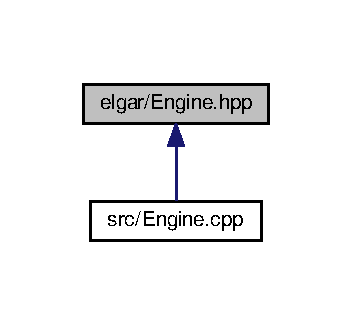
\includegraphics[width=169pt]{Engine_8hpp__dep__incl}
\end{center}
\end{figure}
\subsection*{Classes}
\begin{DoxyCompactItemize}
\item 
class \hyperlink{classelgar_1_1Engine}{elgar\+::\+Engine}
\begin{DoxyCompactList}\small\item\em The \hyperlink{classelgar_1_1Engine}{Engine} class oversees all core functionalities of the Elgar pipeline. Every program using Elgar must utilize this class. (Note\+: Follows the singleton class design pattern) \end{DoxyCompactList}\end{DoxyCompactItemize}
\subsection*{Namespaces}
\begin{DoxyCompactItemize}
\item 
 \hyperlink{namespaceelgar}{elgar}
\end{DoxyCompactItemize}

\hypertarget{Engine_8cpp}{}\section{src/\+Engine.cpp File Reference}
\label{Engine_8cpp}\index{src/\+Engine.\+cpp@{src/\+Engine.\+cpp}}
{\ttfamily \#include \char`\"{}elgar/\+Engine.\+hpp\char`\"{}}\\*
Include dependency graph for Engine.\+cpp\+:
\nopagebreak
\begin{figure}[H]
\begin{center}
\leavevmode
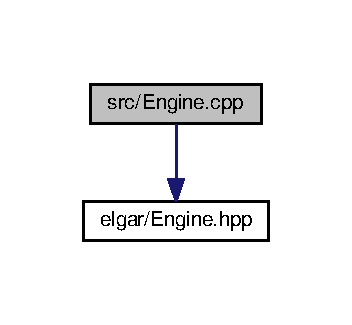
\includegraphics[width=169pt]{Engine_8cpp__incl}
\end{center}
\end{figure}
\subsection*{Namespaces}
\begin{DoxyCompactItemize}
\item 
 \hyperlink{namespaceelgar}{elgar}
\end{DoxyCompactItemize}

%--- End generated contents ---

% Index
\backmatter
\newpage
\phantomsection
\clearemptydoublepage
\addcontentsline{toc}{chapter}{Index}
\printindex

\end{document}
